% XCircuit output "setch.tex" for LaTeX input from setch.ps
\def\putbox#1#2#3#4{\makebox[0in][l]{\makebox[#1][l]{}\raisebox{\baselineskip}[0in][0in]{\raisebox{#2}[0in][0in]{\scalebox{#3}{#4}}}}}
\def\rightbox#1{\makebox[0in][r]{#1}}
\def\centbox#1{\makebox[0in]{#1}}
\def\topbox#1{\raisebox{-0.60\baselineskip}[0in][0in]{#1}}
\def\midbox#1{\raisebox{-0.20\baselineskip}[0in][0in]{#1}}
\begin{center}
   \scalebox{1}{
   \normalsize
   \parbox{4.08333in}{
   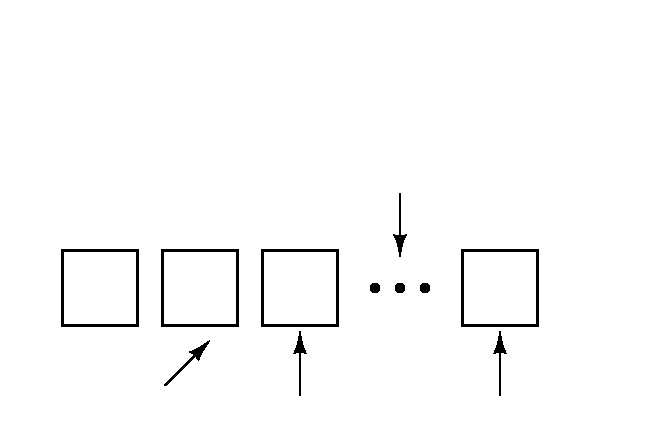
\includegraphics[scale=1,trim= 0 0 0 1.5cm]{../media/setch.ps}\\
   % translate x=544 y=352 scale 0.38
   \putbox{3.39in}{1.72in}{1.20}{}%
   \putbox{0.47in}{1.39in}{1.20}{4}%
   \putbox{3.14in}{1.39in}{1.20}{n}%
   \putbox{3.22in}{0.89in}{1.20}{\centbox{\midbox{0xFF}}}%
   \putbox{0.64in}{0.14in}{1.20}{}%
   \putbox{0.56in}{0.14in}{1.20}{}%
   \putbox{2.89in}{0.06in}{1.20}{Terminador}%
   \putbox{2.31in}{1.56in}{1.20}{Dados}%
   \putbox{4.14in}{1.89in}{1.20}{}%
   \putbox{0.56in}{0.89in}{1.20}{\centbox{\midbox{0x08}}}%
   \putbox{1.14in}{1.39in}{1.20}{5}%
   \putbox{0.39in}{0.06in}{1.20}{Endereco}%
   \putbox{1.81in}{1.39in}{1.20}{6}%
   \putbox{1.56in}{0.06in}{1.20}{Tamanho}%
   \putbox{1.22in}{0.89in}{0.96}{\centbox{\midbox{ADDR}}}%
   \putbox{1.89in}{0.89in}{0.96}{\centbox{\midbox{PSZ}}}%
   \putbox{2.56in}{0.72in}{0.96}{\centbox{\midbox{PRM}}}%
   } % close 'parbox'
   } % close 'scalebox'
   \vspace{-\baselineskip} % this is not necessary, but looks better
\end{center}
